%====================================================================================================
% FaultRecovery: Ampliação da Biblioteca de Tolerância a Falhas
%====================================================================================================
% Apresentação do Trabalho de Conclusão de Curso
%----------------------------------------------------------------------------------------------------
% Autor				: Cleiton Gonçalves de Almeida
% Orientador		: Kleber Kruger
% Instituição 		: UFMS - Universidade Federal do Mato Grosso do Sul
% Campus     		: Coxim
%----------------------------------------------------------------------------------------------------
% Arquivo			: introducao.tex
% Data de criação	: 10 de setembro de 2016
%====================================================================================================

\section{Resultados} \label{Sec:Resultados}

\begin{frame}
	\frametitle{Resultado do Desempenho da Biblioteca FaultRecovery}
	\begin{figure}
		\begin{center}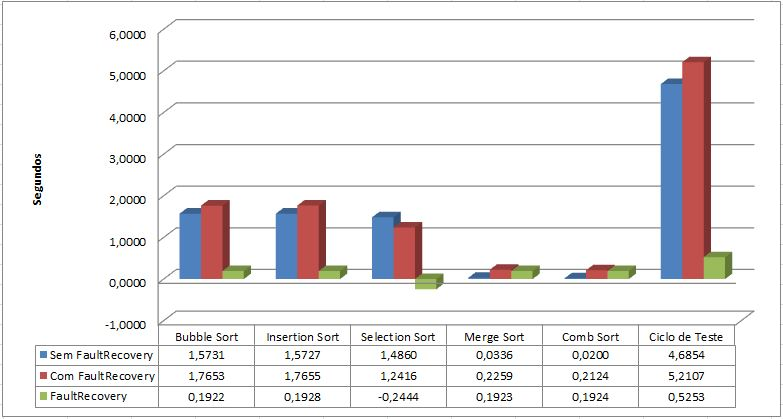
\includegraphics[width=0.92\textwidth]{./figuras/tempoRecovery.png}\end{center}
		\caption{Tempo de execução dos algoritmos de ordenação sem a biblioteca e com ela.}
	\end{figure}
\end{frame}

\begin{frame}
	\frametitle{Resultado do Desempenho da Biblioteca FaultRecovery}
	\begin{figure}
		\begin{center}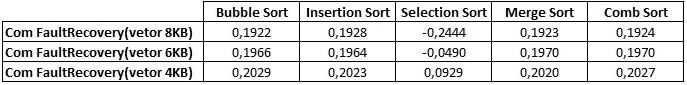
\includegraphics[width=1.0\textwidth]{./figuras/tempoRecovery2.png}\end{center}
		\caption{Tempo de execução da biblioteca FaultRecovery com três	vetores de tamanhos diferentes.}
	\end{figure}
\end{frame}

\begin{frame}
	\frametitle{Eficiência da Classe TData}
	\begin{figure}
		\begin{center}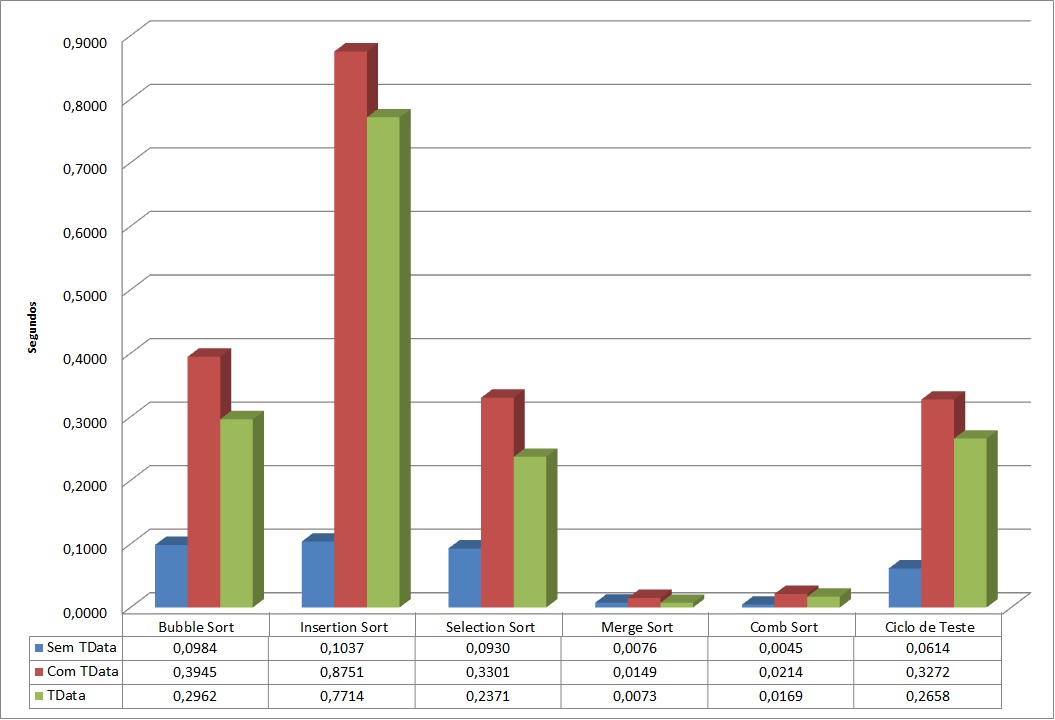
\includegraphics[width=0.8\textwidth]{./figuras/tempoTData.png}\end{center}
		\caption{O tempo de execução dos algoritmos sem a classe TData e com ela.}
	\end{figure}
\end{frame}

\begin{frame}
	\frametitle{Eficiência da Classe TData}
	\begin{figure}
		\begin{center}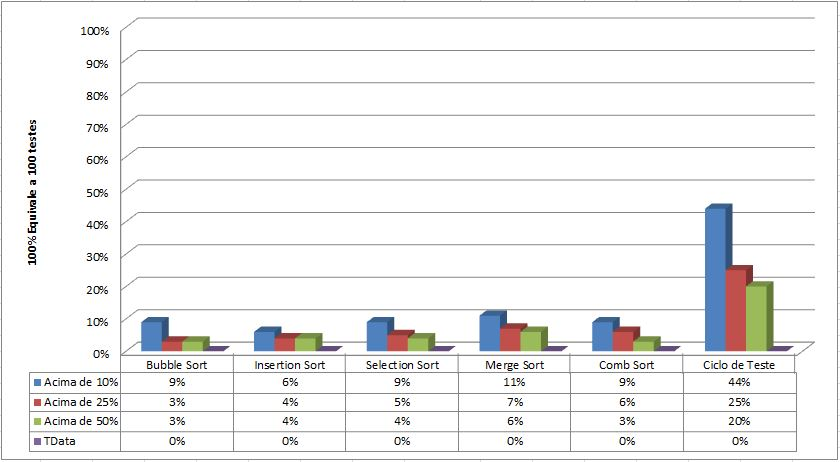
\includegraphics[width=1.0\textwidth]{./figuras/falhaTData.png}\end{center}
		\caption{Falhas detectadas nos teste.}
	\end{figure}
\end{frame}

\begin{frame}
	\frametitle{Recuperação de Falhas da Biblioteca FaultRecovery}
	\begin{figure}
		\begin{center}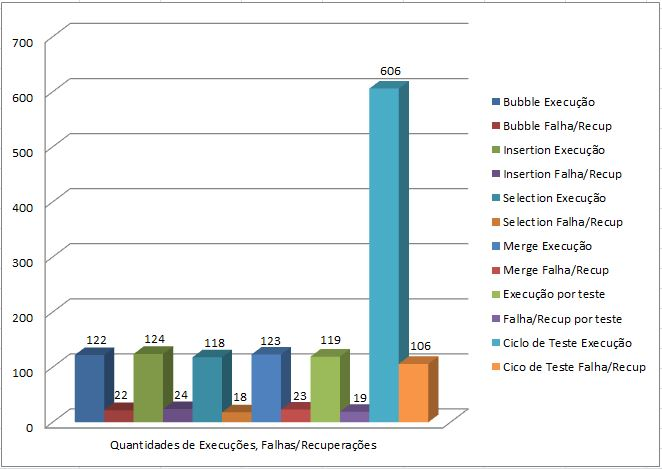
\includegraphics[width=0.82\textwidth]{./figuras/testeFaultRecovery.png}\end{center}
		\caption{Quantidade de execuções e falhas de cada algoritmo.}
	\end{figure}
\end{frame}

\begin{frame}
	\frametitle{Injeção de Falhas na Memória Flash}
	\begin{figure}
		\begin{center}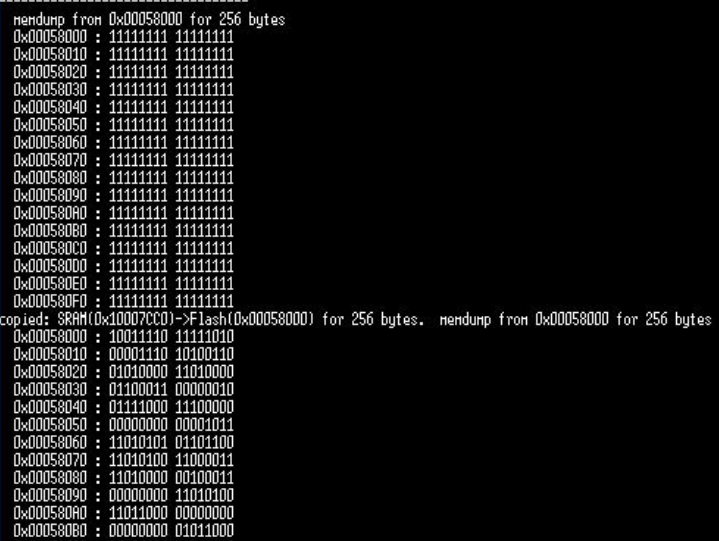
\includegraphics[width=0.72\textwidth]{./figuras/injecaoFlash.png}\end{center}
		\caption{Antes e depois dos bits serem modificados.}
	\end{figure}
\end{frame}
